% mnras_template.tex
%
% LaTeX template for creating an MNRAS paper
%
% v3.0 released 14 May 2015
% (version numbers match those of mnras.cls)
%
% Copyright (C) Royal Astronomical Society 2015
% Authors:
% Keith T. Smith (Royal Astronomical Society)

% Change log
%
% v3.0 May 2015
%    Renamed to match the new package name
%    Version number matches mnras.cls
%    A few minor tweaks to wording
% v1.0 September 2013
%    Beta testing only - never publicly released
%    First version: a simple (ish) template for creating an MNRAS paper

%%%%%%%%%%%%%%%%%%%%%%%%%%%%%%%%%%%%%%%%%%%%%%%%%%
% Basic setup. Most papers should leave these options alone.
\documentclass[a4paper,fleqn,usenatbib]{mnras}

% MNRAS is set in Times font. If you don't have this installed (most LaTeX
% installations will be fine) or prefer the old Computer Modern fonts, comment
% out the following line
%\usepackage{newtxtext,newtxmath}
\usepackage{txfonts}
% Depending on your LaTeX fonts installation, you might get better results with one of these:
%\usepackage{mathptmx}
%\usepackage{txfonts}


% Use vector fonts, so it zooms properly in on-screen viewing software
% Don't change these lines unless you know what you are doing
\usepackage[T1]{fontenc}
\usepackage{ae,aecompl}


%%%%% AUTHORS - PLACE YOUR OWN PACKAGES HERE %%%%%

% Only include extra packages if you really need them. Common packages are:
\usepackage{graphicx}	% Including figure files
\usepackage{amsmath}	% Advanced maths commands
\usepackage{amssymb}	% Extra maths symbols

%%%%%%%%%%%%%%%%%%%%%%%%%%%%%%%%%%%%%%%%%%%%%%%%%%

%%%%% AUTHORS - PLACE YOUR OWN COMMANDS HERE %%%%%

% Please keep new commands to a minimum, and use \newcommand not \def to avoid
% overwriting existing commands. Example:
%\newcommand{\pcm}{\,cm$^{-2}$}	% per cm-squared

%%%%%%%%%%%%%%%%%%%%%%%%%%%%%%%%%%%%%%%%%%%%%%%%%%

%%%%%%%%%%%%%%%%%%% TITLE PAGE %%%%%%%%%%%%%%%%%%%

% Title of the paper, and the short title which is used in the headers.
% Keep the title short and informative.
\title[Quasar Variability]{Solving the puzzle of discrepant variability on monthly time scales implied by SDSS and CRTS datasets}

% The list of authors, and the short list which is used in the headers.
% If you need two or more lines of authors, add an extra line using \newauthor
\author[K. Suberlak et al.]{
Krzysztof Suberlak,$^{1}$\thanks{E-mail: suberlak@uw.edu}
\v{Z}eljko Ivezi\'c, $^{1}$
Chelsea L. MacLeod,$^{2}$
Matthew Graham,$^{3}$ 
\newauthor
$\, \,  $Branimir Sesar$^{4}$
\\
% List of institutions
$^{1}$Department of Astronomy, University of Washington, Seattle, WA, United States\\
$^{2}$Institute for Astronomy, University of Edinburgh, Royal Observatory, Edinburgh, United Kingdom\\
$^{3}$Center for Data-Driven Discovery, California Institute of Technology, Pasadena, CA, United States\\
$^{4}$National Optical Astronomy Observatory, Tucson, AZ, United States.
}

% These dates will be filled out by the publisher
\date{Accepted XXX. Received YYY; in original form ZZZ}

% Enter the current year, for the copyright statements etc.
\pubyear{2015}

% Don't change these lines
\begin{document}
\label{firstpage}
\pagerange{\pageref{firstpage}--\pageref{lastpage}}
\maketitle

% Abstract of the paper
\begin{abstract}

We present improved error analysis for the 3,800 CRTS (Catalina Real-Time Transient Survey) optical quasar light curves from the Sloan Digital Sky Survey Stripe 82 catalog. SDSS time-resolved photometric dataset provided improvement in our understanding of the quasar optical continuum variability. According to SDSS results, the rms variability for small timescales  below 50 days is about 0.06 mag. However,  the more recent CRTS data show about a factor of two larger rms variability for the same spectroscopically confirmed SDSS quasars.  This discrepancy can be resolved if we assume a slight underestimate of photometric errors from the CRTS image processing pipelines. Our detailed analysis of non-variable SDSS standard stars, reobserved by CRTS, reveals that the photometric correction factors of 20-30 \% fully explain the quasar variability. This is consistent with earlier SDSS results.

\end{abstract}

% Select between one and six entries from the list of approved keywords.
% Don't make up new ones.
\begin{keywords}
keyword1 -- keyword2 -- keyword3
\end{keywords}

%%%%%%%%%%%%%%%%%%%%%%%%%%%%%%%%%%%%%%%%%%%%%%%%%%

%%%%%%%%%%%%%%%%% BODY OF PAPER %%%%%%%%%%%%%%%%%%

\section{Introduction}
\label{sec:intro}

Quasar variability is an important characteristic that reveals the structure of innermost region of the accretion disk, and has been the subject of research for the past half century (Matthew, Sandage 1963).   The Sloan Digital Sky Survey (SDSS, Schmidt+2010, Sesar+2007) and Catalina Real-Time Transient Survey (Djorgovski+2012, Drake+2009) allowed unprecedented study of well-calibrated light curves, and draw physical interpretation from the structural form of the variability(Kelly+2009, Kelly+2011, Collier\&Peterson 2001). Damped Random Walk model has been successful in defining the parameters of variability, because it corresponds to a physical situation of an environment where a disturbance is diffused and returns to the median value. Such process has characteristic timescale, corresponding the physical mechanism responsible for variability (Kelly+2009).  Recent SDSS-based studies (MacLeod+2010, Kelly+2009) reflect the traditional timescale of $\tau > 100 $ days in quasar rest frame, supported by OGLE results of Zu+2014 with $ 17 \leq \tau \leq 2700 $ days. However, a CRTS-based study of Graham+2014 that used Slepian Wavelet Variance methodology found $\tau ~ 54$ days. This apparent discrepancy lead us to repeat the analysis of CRTS quasars using a  well-tested approach of the Structure Function (MacLeod+2010, MacLeod+2012, Simonetti+1984, Vanden Berk+2004, Sumi+2005, Bauer+2009). 

Mathematically the structure function relates the flux difference $\Delta m_{ij}$ to time lag $\Delta t_{ji}$  between two points (Schmidt+2010). We investigate the CRTS structure function for standard stars and quasars. We find that non-variable stars exhibit nonzero structure function, which can be remedied by assuming an error underestimate. Adjusting the CRTS error by an appropriate correction factor $f_{c}$ we reproduce the expected non-variable behavior for stars. Performing a detailed analysis of all points that contribute to the  $\Delta t < 50$ days part of structure function we find no trace of very short ensemble characteristic timescales of $\tau \approx 54$ days. 
 
In this work we present the detailed error analysis of CRTS and SDSS data. In section \ref{sec:obs} we describe the properties of our dataset, all selection criteria, and the structure function analysis.  In section \ref{sec:err_analysis} we explain the results of our analysis of the small timescale subset of the structure function. This is followed by discussion of the impact of our result, and conclusions in sections \ref{sec:discussion} and \ref{sec:conclusions}.
 

\section{Observations}
\label{sec:obs}

\subsection{Data overview}

The CRTS survey (Drake+2009) telescopes use 4kx4k CCDs, observations are made in unfiltered white light (Djorgovski+2011).  As part of the CRTS pipeline this unfiltered photometry is calibrated to the V-band zero point. Our CRTS Quasar sample consists of 7754 Quasars, and after selecting only those that have more than 10 measurements, the sample is reduced to 7707 objects. Within that sample , $96 \% $ observations span the time of $7-9$ years. The light curve and sample-averaged mean and median error is $0.22$. The mean and median brightness is $19.50$ and  $19.66$ respectively. The mean number of individual observations per light curve  is $209$. $91.2\%$ (7035 of 7707) quasars were observed between 1 to 4 times per night.  (See Fig.\ref{fig:CRTS_QSO_stats})

We complement the CRTS Quasars with information from position-matched SDSS Stripe 82 catalog[reference]. The catalog includes SDSS DR7 stripe 82 ($22h 24m < R.A. < 04h 08m$ and $| Dec | < 1.27 deg$) spectroscopically confirmed  8,974 quasars cross-matched with 2MASS photometry. 

\begin{figure}
\label{fig:CRTS_QSO_stats}
 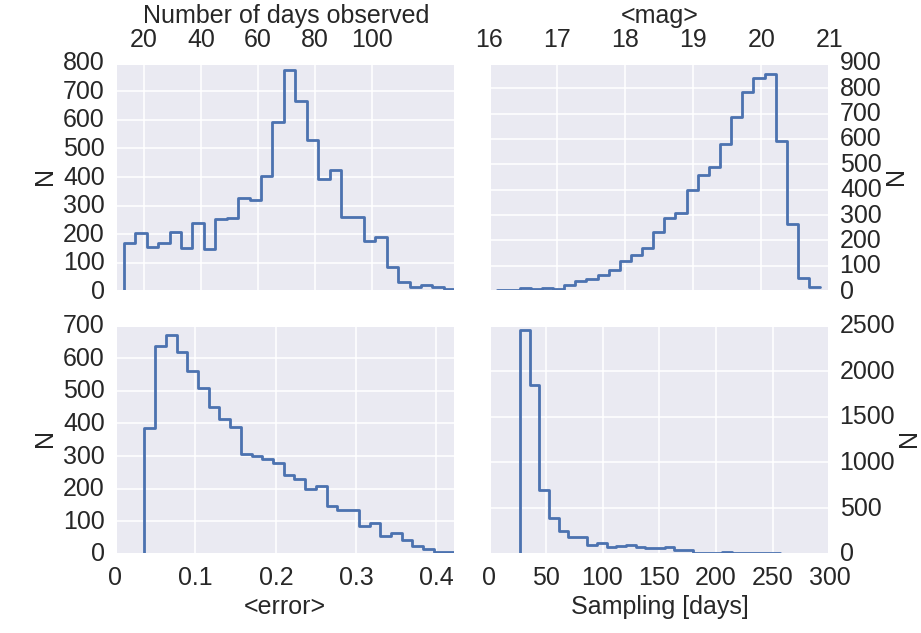
\includegraphics[width=\columnwidth]{Fig_1_Stats_CRTS_QSO_used.png}
 \caption{Statistical information about the CRTS Quasar sample including 7601 day-averaged light curves. The upper-left panel shows the number of days that a given quasar was observed, i.e. $max(MJD)-min(MJD)$ per light curve. The upper-right panel shows the average light curve magnitude. The bottom-left panel shows the light curve averaged error. If $i$, $i+1$ are two consecutive day-averaged observations in the light curve, then $MJD_{i} - MJD_{i+1}$ is the sampling interval. The bottom-right panel shows light curve - averaged sampling intervals.}
\end{figure}

As a control sample we use CRTS observations of standard stars in Stripe 82. Those are  complemented with the SDSS photometry (Ivezic+2007) - we positionally  match the CRTS observations to the SDSS calibration stars catalog (ver.2.6). 


\subsection{Day-averaging and selection}
\label{sec:sample_sel}


To improve signal-to-noise ratio CRTS light curves were day-averaged.  Denoting individual CRTS reported measurement error as $e_{i}$, the combined error $e_{w}$ consists of the sum of weighted errors where weight for each point is $ w_{i} = 1 / e_{i}^{2}$ (see eq.\ref{eq:day_averaging}). 


\begin{equation}
\label{eq:day_averaging}
 e_{w} = \frac{1}{\sqrt[]{\sum_{i} w_{i}}}
\end{equation}

If the resulting $e_{w}$ was smaller than $0.02$ $mag$, then  $0.01$ $mag$ was added in quadrature. For further analysis we selected light curves that had more than $10$ observation days, which reduced the sample to $7601$ CRTS Quasars. A typical sampling interval of day-averaged CRTS Quasar lightcurves is $\approx 20$ days. 

\subsection{Structure Function analysis}

 The structure function is a well-studied characteristic of quasar light curves, embodying the relationship between the time lag and the amplitude of brightness variability (Cristiani+1996, Schmidt+2010, Vanden Berk +2004, de Vries + 2005, Rengstorf + 2006). Similarly to Schmidt+2010, we  calculate the structure function using  the magnitude difference $\Delta m _{i,j}$ between light curve points $i$ and $j$, separated by a time lag $\Delta t_{i,j}$. To avoid the additional uncertainty of redshift estimates based on the SDSS spectra, we also use time lags in the observed frame. We add the error information in quadrature: $e_{ij} = \sqrt{e_{i}^{2}+e_{j}^{2}}$.

To ensure a uniform sample we impose the following selection criteria, based on the SDSS r-band photometry: for CRTS quasars  $17< m_{SDSS,r} < 20$, and the CRTS lightcurve-averaged error to be  $0.05 < \langle CRTS_{err} \rangle < 0.3$. Similarly, for the CRTS standard stars, $17 < m_{SDSS,r} < 20 $, and the lightcurve-averaged error $0.05 < \langle CRTS_{err} \rangle < 0.3$. Based on the SDSS photometry in $g$ and $i$ filters  we divide the comparison stars into two color bins: "red" with   $1 < g-i < 3$ and "blue" $-1 < g-i < 1$. 

To analyze the magnitude difference data we bin it in logarithmic time lag space. The number of chosen bins is a choice of convenience between very coarse grid (a small number of bins) or a very fine grid, risking a small number of points per bin. Having performed tests  with $50$, $100$, $200$, $400$ bins we find that $200$ is the right choice between computational efficiency and preservation of scientific information. For each bin we calculate four statistics, shown on Fig.~\ref{fig:panel_plots}: Standard deviation ($\sigma$, Gaussian robust deviation from the mean $\sigma_{G}=0.7414 (q_{75}-q_{25})$, Structure Function ($SF$) and the mean ($\mu$).  We calculate the $SF$ using an exact prescription involving marginalizing the log-likelihood of the probability in $p(SF)$ and $p(\mu)$ space per bin, after [Ivezic+2013], chapter 5: 
 
\begin{equation}
\centering
\frac{d p(SF}{d SF } \bigg| _{SF = mode} = 0
\end{equation}

To show the departure of raw CRTS quasar points we fit to the $SF$ a  fiducial Damped Random Walk model:
\begin{equation}
SF(\Delta t) = SF_{\infty} \cdot \left( 1-e^{-\Delta t / \tau} \right) ^ {1/2}
\end{equation}

with model error $\sqrt{SF(\Delta t) ^ {2} + err_{SF} ^ {2}}$. 

Note how both blue and red stars do not exhibit signs of variability as expected, whereas quasars (black) clearly show an intrinsic variability. At the low timescales $\log{\tau} < 1.7$ CRTS quasar $SF$ departs from the fiducial model of Structure Function. 
If this was caused by an error underestimate, the variability on short timescales would be reduced by incorporating an error correction factor $f_{c}$. We find that simple increase of CRTS errors by $30\%$ leads to a reduction of quasar $SF$  to zero (see Fig.~\ref{fig:SF_panel}). This prompted a more detailed error analysis of points involved in short timescales on the plot, described in Sec.\ref{sec:err_analysis}. 
 


\begin{figure}
\label{fig:panel_plots}
 \includegraphics[width=\columnwidth]{{Fig_2_18.5-19_panels_fc-1.0}.png}
 \caption{The four panels show statistics calculated for the subsample of 333 CRTS quasars (black points), 1400 "blue" stars (blue points), and 2087 "red" stars (red points), all  chosen according to the SDSS r magnitude $18.5 < m < 19$.  For "red"  stars we require that SDSS colors are $1 < g-i < 3$ and  for "blue" stars $-1 < g-i < 1$. Lightcurve-derived  pairwise brightness differences for all objects of a given type are binned according to  linearly spaced $200$ bins in $\Delta_{t}$. The binning was not found to affect the main features of the plot.  The sine-like modulation reflects differences in number of points in each bin (from tens to hundreds of thousands per bin). For each bin, we calculated for each type of object the standard deviation $\sigma_{stdev}$, the robust Gaussian standard deviation $\sigma_{G}$ (from the interquartile range $0.7414 (q_{75}-q_{25}$), Structure Function and the mean(using eqs.$5.67-5.68$ in $Ivezic+2004$ (the AstroML book). Yellow dashed line on the SF panel traces the fiducial Damped Random Walk model. }
\end{figure}

\begin{figure}
\label{fig:SF_panel}
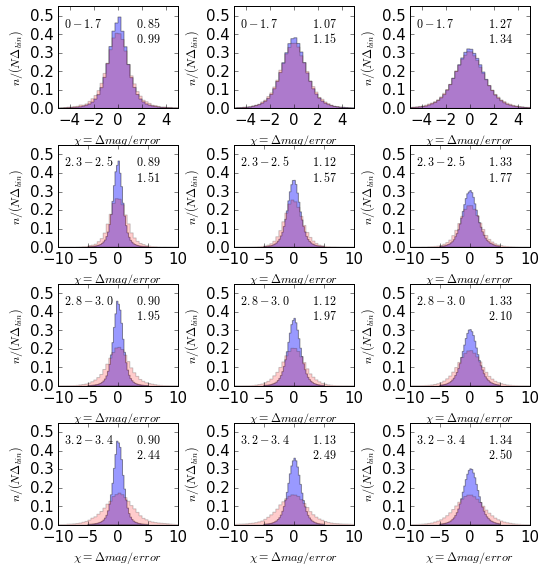
\includegraphics[width=1.1\columnwidth]{Fig_3_histogram_panels.png}
 \caption{The top panels show how the histogram of  $\chi = \Delta_{m}/ \mathrm{error}$ for small 
timescales ($\log{\Delta_{t}} < 1.7$, $t<50$ days) for  quasars (red) overlaps almost perfectly with blue stars (blue). The  implied small quasar variability is at the level  measured by SDSS.  From left to right, we iterate over the  magnitude bins :  $17-18$,  $18-18.5$, and $18.5-19$ mag. From top to bottom we change the  $\log{\Delta_{t}}$  range. Note how  the  stars, being nonvariable, maintain the same spread of $\chi$, due to their lack of intrinsic variability. The quasars spread more thanks to their intrinsic variability, but at small timescales their spread is same as that of stars, consistent with their lack of short timescale variability. On each plot numbers in the upper-left corner indicate the $\log{\Delta_{t}}$ range, and in the upper-right the robust width of stellar and quasar distributions of $\chi$. }
\end{figure}

\section{Results of detailed sample error analysis}
\label{sec:err_analysis}

To analyze the error properties of the short time lag points we select $\log{\tau} < 1.7$ points for CRTS quasars and stars, which includes $721 283$ time-lag points based on quasars, and $314 248$ time-lag  stellar points. To disentangle the magnitude sensitivity, we further split the sample into  three  magnitude bins : $17-18$,  $18-18.5$ and $18.5-19$ $^{mag}$. 


We separate contributions from the intrinsic variability and the error-related variance by comparing CRTS stars to quasars. Assuming that each $\delta m$ data point originates from a homoscedastic Gaussian distribution, with a standard deviation $\sigma_{com}$ (that includes all intrinsic variability $\sigma$ and error-related $f_{c}*e_{i}$):

\begin{equation}
    \sigma_{com} = \sqrt[]{\sigma^{2} + \left( f_{c} \cdot e_{i}   \right) ^ {2}}
\label{eq:sig_comb}
\end{equation}

and the mean $\mu$, then the distribution of all magnitude difference points in our sample is a sum of Gaussians:

\begin{equation}
     \frac{1}{N}.\sum_{i=0}^{N} \frac{1}{\sqrt[]{2 \pi} \sigma_{com}} . e ^ {-\left( x_{i} - \mu \right)^{2} / \left( 2 \sigma_{com}^{2} \right) }
	\label{eq:comb_gaussians}
\end{equation}
Since standard stars do not vary on level above $0.02 mag$ [reference],  it is reasonable to assume for stars $\sigma=0$, and a distribution centered around $\mu=0$. With these parameters we fit the ensemble of Gaussian distributions per magnitude bin  to a histogram of "blue" stars to recover an error correction factor that would explain the variability ($\sigma_{com} = f_{c} \cdot e_{i}$. Those factors applied to quasar distribution explain their variability (see Figs. ~\ref{fig:CRTS_QSO_sample} and ~\ref{fig:CRTS_StarB_sample}). 


\begin{figure}
\label{fig:CRTS_QSO_sample}
 \includegraphics[width=\columnwidth]{{Fig_4_SF_QSO_starsB_r_cut_fc-0.863-1.091-1.3}.png}
 \caption{Three panels compare the Structure Function (SF)  for quasars and blue stars in three bins based on their mean SDSS $r$ magnitude. We correct CRTS errors using listed $fc$ factors. Stars have a flat SF consistent with their lack of  variability, whereas quasars have a nonzero variability. At short time scales, the quasar variability seen in CRTS data is consistent with that from SDSS, shown by horizontal green lines. }
\end{figure}


\section{Discussion}
\label{sec:discussion}

\section{Conclusions}
\label{sec:conclusions}
CRTS errors were underestimated at the 20-30 \% level.

Implications:  * information from correspondence with M. Graham  
* other recent findings that are based on short timescale CRTS variability  - all would be called into question  



\section*{Acknowledgements}

Funding for the SDSS and SDSS-II has been provided by the Alfred P. Sloan Foundation, the Participating Institutions, the National Science Foundation, the U.S. Department of Energy, the National Aeronautics and Space Administration, the Japanese Monbukagakusho, the Max Planck Society, and the Higher Education Funding Council for England. The SDSS Web Site is http://www.sdss.org/.

The SDSS is managed by the Astrophysical Research Consortium for the Participating Institutions. The Participating Institutions are the American Museum of Natural History, Astrophysical Institute Potsdam, University of Basel, University of Cambridge, Case Western Reserve University, University of Chicago, Drexel University, Fermilab, the Institute for Advanced Study, the Japan Participation Group, Johns Hopkins University, the Joint Institute for Nuclear Astrophysics, the Kavli Institute for Particle Astrophysics and Cosmology, the Korean Scientist Group, the Chinese Academy of Sciences (LAMOST), Los Alamos National Laboratory, the Max-Planck-Institute for Astronomy (MPIA), the Max-Planck-Institute for Astrophysics (MPA), New Mexico State University, Ohio State University, University of Pittsburgh, University of Portsmouth, Princeton University, the United States Naval Observatory, and the University of Washington. 


%%%%%%%%%%%%%%%%%%%%%%%%%%%%%%%%%%%%%%%%%%%%%%%%%%

%%%%%%%%%%%%%%%%%%%% REFERENCES %%%%%%%%%%%%%%%%%%

% The best way to enter references is to use BibTeX:

%\bibliographystyle{mnras}
%\bibliography{example} % if your bibtex file is called example.bib

%%%%%%%%%%%%%%%%%%%%%%%%%%%%%%%%%%%%%%%%%%%%%%%%%%


% Don't change these lines
\bsp	% typesetting comment
\label{lastpage}
\end{document}

% End of mnras_template.tex
